\documentclass[1p]{elsarticle_modified}
%\bibliographystyle{elsarticle-num}

%\usepackage[colorlinks]{hyperref}
%\usepackage{abbrmath_seonhwa} %\Abb, \Ascr, \Acal ,\Abf, \Afrak
\usepackage{amsfonts}
\usepackage{amssymb}
\usepackage{amsmath}
\usepackage{amsthm}
\usepackage{scalefnt}
\usepackage{amsbsy}
\usepackage{kotex}
\usepackage{caption}
\usepackage{subfig}
\usepackage{color}
\usepackage{graphicx}
\usepackage{xcolor} %% white, black, red, green, blue, cyan, magenta, yellow
\usepackage{float}
\usepackage{setspace}
\usepackage{hyperref}

\usepackage{tikz}
\usetikzlibrary{arrows}

\usepackage{multirow}
\usepackage{array} % fixed length table
\usepackage{hhline}

%%%%%%%%%%%%%%%%%%%%%
\makeatletter
\renewcommand*\env@matrix[1][\arraystretch]{%
	\edef\arraystretch{#1}%
	\hskip -\arraycolsep
	\let\@ifnextchar\new@ifnextchar
	\array{*\c@MaxMatrixCols c}}
\makeatother %https://tex.stackexchange.com/questions/14071/how-can-i-increase-the-line-spacing-in-a-matrix
%%%%%%%%%%%%%%%

\usepackage[normalem]{ulem}

\newcommand{\msout}[1]{\ifmmode\text{\sout{\ensuremath{#1}}}\else\sout{#1}\fi}
%SOURCE: \msout is \stkout macro in https://tex.stackexchange.com/questions/20609/strikeout-in-math-mode

\newcommand{\cancel}[1]{
	\ifmmode
	{\color{red}\msout{#1}}
	\else
	{\color{red}\sout{#1}}
	\fi
}

\newcommand{\add}[1]{
	{\color{blue}\uwave{#1}}
}

\newcommand{\replace}[2]{
	\ifmmode
	{\color{red}\msout{#1}}{\color{blue}\uwave{#2}}
	\else
	{\color{red}\sout{#1}}{\color{blue}\uwave{#2}}
	\fi
}

\newcommand{\Sol}{\mathcal{S}} %segment
\newcommand{\D}{D} %diagram
\newcommand{\A}{\mathcal{A}} %arc


%%%%%%%%%%%%%%%%%%%%%%%%%%%%%5 test

\def\sl{\operatorname{\textup{SL}}(2,\Cbb)}
\def\psl{\operatorname{\textup{PSL}}(2,\Cbb)}
\def\quan{\mkern 1mu \triangleright \mkern 1mu}

\theoremstyle{definition}
\newtheorem{thm}{Theorem}[section]
\newtheorem{prop}[thm]{Proposition}
\newtheorem{lem}[thm]{Lemma}
\newtheorem{ques}[thm]{Question}
\newtheorem{cor}[thm]{Corollary}
\newtheorem{defn}[thm]{Definition}
\newtheorem{exam}[thm]{Example}
\newtheorem{rmk}[thm]{Remark}
\newtheorem{alg}[thm]{Algorithm}

\newcommand{\I}{\sqrt{-1}}
\begin{document}

%\begin{frontmatter}
%
%\title{Boundary parabolic representations of knots up to 8 crossings}
%
%%% Group authors per affiliation:
%\author{Yunhi Cho} 
%\address{Department of Mathematics, University of Seoul, Seoul, Korea}
%\ead{yhcho@uos.ac.kr}
%
%
%\author{Seonhwa Kim} %\fnref{s_kim}}
%\address{Center for Geometry and Physics, Institute for Basic Science, Pohang, 37673, Korea}
%\ead{ryeona17@ibs.re.kr}
%
%\author{Hyuk Kim}
%\address{Department of Mathematical Sciences, Seoul National University, Seoul 08826, Korea}
%\ead{hyukkim@snu.ac.kr}
%
%\author{Seokbeom Yoon}
%\address{Department of Mathematical Sciences, Seoul National University, Seoul, 08826,  Korea}
%\ead{sbyoon15@snu.ac.kr}
%
%\begin{abstract}
%We find all boundary parabolic representation of knots up to 8 crossings.
%
%\end{abstract}
%\begin{keyword}
%    \MSC[2010] 57M25 
%\end{keyword}
%
%\end{frontmatter}

%\linenumbers
%\tableofcontents
%
\newcommand\colored[1]{\textcolor{white}{\rule[-0.35ex]{0.8em}{1.4ex}}\kern-0.8em\color{red} #1}%
%\newcommand\colored[1]{\textcolor{white}{ #1}\kern-2.17ex	\textcolor{white}{ #1}\kern-1.81ex	\textcolor{white}{ #1}\kern-2.15ex\color{red}#1	}

{\Large $\underline{12a_{1244}~(K12a_{1244})}$}

\setlength{\tabcolsep}{10pt}
\renewcommand{\arraystretch}{1.6}
\vspace{1cm}\begin{tabular}{m{100pt}>{\centering\arraybackslash}m{274pt}}
\multirow{5}{120pt}{
	\centering
	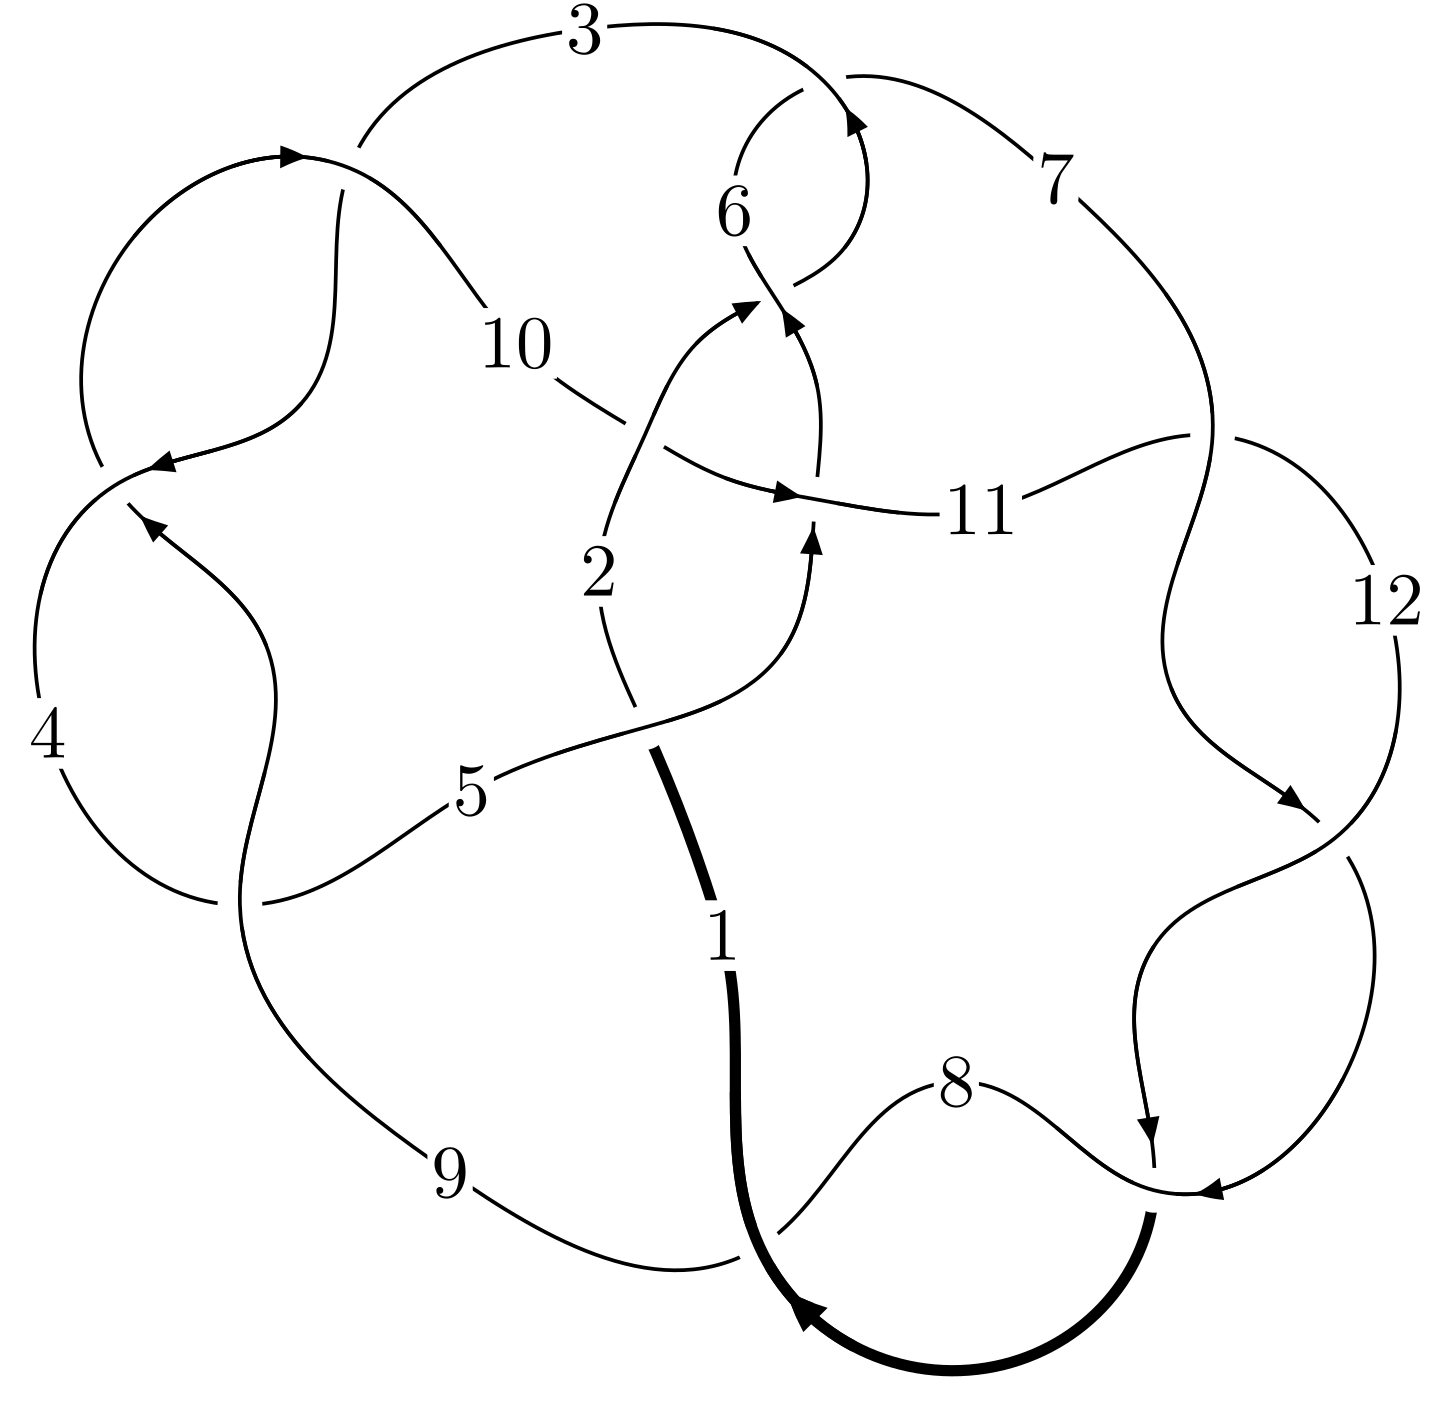
\includegraphics[width=112pt]{../../../GIT/diagram.site/Diagrams/png/2045_12a_1244.png}\\
\ \ \ A knot diagram\footnotemark}&
\allowdisplaybreaks
\textbf{Linearized knot diagam} \\
\cline{2-2}
 &
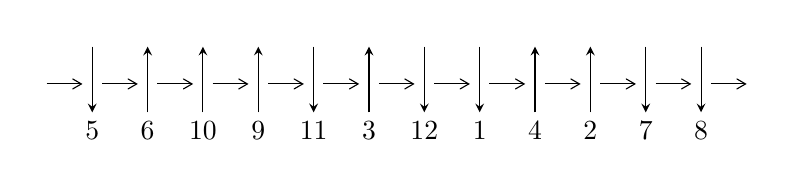
\begin{tikzpicture}[x=20pt, y=17pt]
	% nodes
	\node (C0) at (0, 0) {};
	\node (C1) at (1, 0) {};
	\node (C1U) at (1, +1) {};
	\node (C1D) at (1, -1) {5};

	\node (C2) at (2, 0) {};
	\node (C2U) at (2, +1) {};
	\node (C2D) at (2, -1) {6};

	\node (C3) at (3, 0) {};
	\node (C3U) at (3, +1) {};
	\node (C3D) at (3, -1) {10};

	\node (C4) at (4, 0) {};
	\node (C4U) at (4, +1) {};
	\node (C4D) at (4, -1) {9};

	\node (C5) at (5, 0) {};
	\node (C5U) at (5, +1) {};
	\node (C5D) at (5, -1) {11};

	\node (C6) at (6, 0) {};
	\node (C6U) at (6, +1) {};
	\node (C6D) at (6, -1) {3};

	\node (C7) at (7, 0) {};
	\node (C7U) at (7, +1) {};
	\node (C7D) at (7, -1) {12};

	\node (C8) at (8, 0) {};
	\node (C8U) at (8, +1) {};
	\node (C8D) at (8, -1) {1};

	\node (C9) at (9, 0) {};
	\node (C9U) at (9, +1) {};
	\node (C9D) at (9, -1) {4};

	\node (C10) at (10, 0) {};
	\node (C10U) at (10, +1) {};
	\node (C10D) at (10, -1) {2};

	\node (C11) at (11, 0) {};
	\node (C11U) at (11, +1) {};
	\node (C11D) at (11, -1) {7};

	\node (C12) at (12, 0) {};
	\node (C12U) at (12, +1) {};
	\node (C12D) at (12, -1) {8};
	\node (C13) at (13, 0) {};

	% arrows
	\draw[->,>={angle 60}]
	(C0) edge (C1) (C1) edge (C2) (C2) edge (C3) (C3) edge (C4) (C4) edge (C5) (C5) edge (C6) (C6) edge (C7) (C7) edge (C8) (C8) edge (C9) (C9) edge (C10) (C10) edge (C11) (C11) edge (C12) (C12) edge (C13) ;	\draw[->,>=stealth]
	(C1U) edge (C1D) (C2D) edge (C2U) (C3D) edge (C3U) (C4D) edge (C4U) (C5U) edge (C5D) (C6D) edge (C6U) (C7U) edge (C7D) (C8U) edge (C8D) (C9D) edge (C9U) (C10D) edge (C10U) (C11U) edge (C11D) (C12U) edge (C12D) ;
	\end{tikzpicture} \\
\hhline{~~} \\& 
\textbf{Solving Sequence} \\ \cline{2-2} 
 &
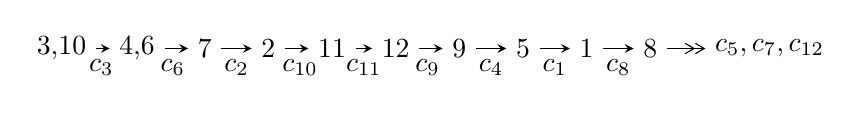
\begin{tikzpicture}[x=23pt, y=7pt]
	% node
	\node (A0) at (-1/8, 0) {3,10};
	\node (A1) at (17/16, 0) {4,6};
	\node (A2) at (17/8, 0) {7};
	\node (A3) at (25/8, 0) {2};
	\node (A4) at (33/8, 0) {11};
	\node (A5) at (41/8, 0) {12};
	\node (A6) at (49/8, 0) {9};
	\node (A7) at (57/8, 0) {5};
	\node (A8) at (65/8, 0) {1};
	\node (A9) at (73/8, 0) {8};
	\node (C1) at (1/2, -1) {$c_{3}$};
	\node (C2) at (13/8, -1) {$c_{6}$};
	\node (C3) at (21/8, -1) {$c_{2}$};
	\node (C4) at (29/8, -1) {$c_{10}$};
	\node (C5) at (37/8, -1) {$c_{11}$};
	\node (C6) at (45/8, -1) {$c_{9}$};
	\node (C7) at (53/8, -1) {$c_{4}$};
	\node (C8) at (61/8, -1) {$c_{1}$};
	\node (C9) at (69/8, -1) {$c_{8}$};
	\node (A10) at (11, 0) {$c_{5},c_{7},c_{12}$};

	% edge
	\draw[->,>=stealth]	
	(A0) edge (A1) (A1) edge (A2) (A2) edge (A3) (A3) edge (A4) (A4) edge (A5) (A5) edge (A6) (A6) edge (A7) (A7) edge (A8) (A8) edge (A9) ;
	\draw[->>,>={angle 60}]	
	(A9) edge (A10);
\end{tikzpicture} \\ 

\end{tabular} \\

\footnotetext{
The image of knot diagram is generated by the software ``\textbf{Draw programme}" developed by Andrew Bartholomew(\url{http://www.layer8.co.uk/maths/draw/index.htm\#Running-draw}), where we modified some parts for our purpose(\url{https://github.com/CATsTAILs/LinksPainter}).
}\phantom \\ \newline 
\centering \textbf{Ideals for irreducible components\footnotemark of $X_{\text{par}}$} 
 
\begin{align*}
I^u_{1}&=\langle 
5.55213\times10^{84} u^{75}-1.16390\times10^{85} u^{74}+\cdots+5.41696\times10^{85} b+4.82475\times10^{85},\\
\phantom{I^u_{1}}&\phantom{= \langle  }5.54157\times10^{84} u^{75}-2.95347\times10^{84} u^{74}+\cdots+5.41696\times10^{85} a-3.16627\times10^{86},\;u^{76}- u^{75}+\cdots+4 u-8\rangle \\
I^u_{2}&=\langle 
- u^{16}-9 u^{14}-31 u^{12}- u^{11}-49 u^{10}-6 u^9-31 u^8-12 u^7-9 u^5+4 u^4-2 u^3+u^2+b- u+1,\\
\phantom{I^u_{2}}&\phantom{= \langle  }u^{16}+u^{15}+10 u^{14}+9 u^{13}+40 u^{12}+33 u^{11}+81 u^{10}+63 u^9+86 u^8+66 u^7+44 u^6+36 u^5+9 u^4+8 u^3+a-2,\\
\phantom{I^u_{2}}&\phantom{= \langle  }u^{17}+10 u^{15}+40 u^{13}+u^{12}+80 u^{11}+7 u^{10}+80 u^9+18 u^8+31 u^7+21 u^6-4 u^5+11 u^4-5 u^3+3 u^2-2 u+1\rangle \\
\\
\end{align*}
\raggedright * 2 irreducible components of $\dim_{\mathbb{C}}=0$, with total 93 representations.\\
\footnotetext{All coefficients of polynomials are rational numbers. But the coefficients are sometimes approximated in decimal forms when there is not enough margin.}
\newpage
\renewcommand{\arraystretch}{1}
\centering \section*{I. $I^u_{1}= \langle 5.55\times10^{84} u^{75}-1.16\times10^{85} u^{74}+\cdots+5.42\times10^{85} b+4.82\times10^{85},\;5.54\times10^{84} u^{75}-2.95\times10^{84} u^{74}+\cdots+5.42\times10^{85} a-3.17\times10^{86},\;u^{76}- u^{75}+\cdots+4 u-8 \rangle$}
\flushleft \textbf{(i) Arc colorings}\\
\begin{tabular}{m{7pt} m{180pt} m{7pt} m{180pt} }
\flushright $a_{3}=$&$\begin{pmatrix}1\\0\end{pmatrix}$ \\
\flushright $a_{10}=$&$\begin{pmatrix}0\\u\end{pmatrix}$ \\
\flushright $a_{4}=$&$\begin{pmatrix}1\\- u^2\end{pmatrix}$ \\
\flushright $a_{6}=$&$\begin{pmatrix}-0.102300 u^{75}+0.0545226 u^{74}+\cdots-6.18614 u+5.84511\\-0.102495 u^{75}+0.214862 u^{74}+\cdots+6.25886 u-0.890674\end{pmatrix}$ \\
\flushright $a_{7}=$&$\begin{pmatrix}-0.204796 u^{75}+0.269385 u^{74}+\cdots+0.0727163 u+4.95443\\-0.102495 u^{75}+0.214862 u^{74}+\cdots+6.25886 u-0.890674\end{pmatrix}$ \\
\flushright $a_{2}=$&$\begin{pmatrix}0.108222 u^{75}-0.118173 u^{74}+\cdots-13.2901 u-1.23742\\0.0265752 u^{75}-0.118287 u^{74}+\cdots-5.18142 u-0.132099\end{pmatrix}$ \\
\flushright $a_{11}=$&$\begin{pmatrix}0.179021 u^{75}-0.179939 u^{74}+\cdots-9.84024 u-0.938082\\0.0355776 u^{75}-0.0834769 u^{74}+\cdots-1.36926 u-0.250356\end{pmatrix}$ \\
\flushright $a_{12}=$&$\begin{pmatrix}0.192907 u^{75}-0.137353 u^{74}+\cdots-9.43677 u-5.08532\\0.0863896 u^{75}-0.0566665 u^{74}+\cdots-10.9587 u-0.256097\end{pmatrix}$ \\
\flushright $a_{9}=$&$\begin{pmatrix}- u\\u^3+u\end{pmatrix}$ \\
\flushright $a_{5}=$&$\begin{pmatrix}u^2+1\\- u^4-2 u^2\end{pmatrix}$ \\
\flushright $a_{1}=$&$\begin{pmatrix}0.0664020 u^{75}-0.174533 u^{74}+\cdots-16.3898 u-1.57130\\-0.0196414 u^{75}-0.0913926 u^{74}+\cdots-5.73736 u-0.0549055\end{pmatrix}$ \\
\flushright $a_{8}=$&$\begin{pmatrix}0.272464 u^{75}-0.292969 u^{74}+\cdots-18.6154 u-3.01996\\0.155586 u^{75}-0.133803 u^{74}+\cdots-10.7797 u-0.765404\end{pmatrix}$\\&\end{tabular}
\flushleft \textbf{(ii) Obstruction class $= -1$}\\~\\
\flushleft \textbf{(iii) Cusp Shapes $= 0.175958 u^{75}-0.0797037 u^{74}+\cdots+21.9858 u+2.71207$}\\~\\
\newpage\renewcommand{\arraystretch}{1}
\flushleft \textbf{(iv) u-Polynomials at the component}\newline \\
\begin{tabular}{m{50pt}|m{274pt}}
Crossings & \hspace{64pt}u-Polynomials at each crossing \\
\hline $$\begin{aligned}c_{1}\end{aligned}$$&$\begin{aligned}
&u^{76}+5 u^{75}+\cdots+5251032 u+1662433
\end{aligned}$\\
\hline $$\begin{aligned}c_{2},c_{6}\end{aligned}$$&$\begin{aligned}
&u^{76}-20 u^{74}+\cdots-13 u+1
\end{aligned}$\\
\hline $$\begin{aligned}c_{3},c_{4},c_{9}\end{aligned}$$&$\begin{aligned}
&u^{76}+u^{75}+\cdots-4 u-8
\end{aligned}$\\
\hline $$\begin{aligned}c_{5}\end{aligned}$$&$\begin{aligned}
&u^{76}+u^{75}+\cdots-39 u+19
\end{aligned}$\\
\hline $$\begin{aligned}c_{7},c_{8},c_{11}\\c_{12}\end{aligned}$$&$\begin{aligned}
&u^{76}- u^{75}+\cdots-122 u-19
\end{aligned}$\\
\hline $$\begin{aligned}c_{10}\end{aligned}$$&$\begin{aligned}
&u^{76}-4 u^{75}+\cdots+14 u+1
\end{aligned}$\\
\hline
\end{tabular}\\~\\
\newpage\renewcommand{\arraystretch}{1}
\flushleft \textbf{(v) Riley Polynomials at the component}\newline \\
\begin{tabular}{m{50pt}|m{274pt}}
Crossings & \hspace{64pt}Riley Polynomials at each crossing \\
\hline $$\begin{aligned}c_{1}\end{aligned}$$&$\begin{aligned}
&y^{76}-39 y^{75}+\cdots-83103653061344 y+2763683479489
\end{aligned}$\\
\hline $$\begin{aligned}c_{2},c_{6}\end{aligned}$$&$\begin{aligned}
&y^{76}-40 y^{75}+\cdots-75 y+1
\end{aligned}$\\
\hline $$\begin{aligned}c_{3},c_{4},c_{9}\end{aligned}$$&$\begin{aligned}
&y^{76}+83 y^{75}+\cdots+1264 y+64
\end{aligned}$\\
\hline $$\begin{aligned}c_{5}\end{aligned}$$&$\begin{aligned}
&y^{76}-5 y^{75}+\cdots-7791 y+361
\end{aligned}$\\
\hline $$\begin{aligned}c_{7},c_{8},c_{11}\\c_{12}\end{aligned}$$&$\begin{aligned}
&y^{76}-97 y^{75}+\cdots-10590 y+361
\end{aligned}$\\
\hline $$\begin{aligned}c_{10}\end{aligned}$$&$\begin{aligned}
&y^{76}+60 y^{74}+\cdots-172 y+1
\end{aligned}$\\
\hline
\end{tabular}\\~\\
\newpage\flushleft \textbf{(vi) Complex Volumes and Cusp Shapes}
$$\begin{array}{c|c|c}  
\text{Solutions to }I^u_{1}& \I (\text{vol} + \sqrt{-1}CS) & \text{Cusp shape}\\
 \hline 
\begin{aligned}
u &= \phantom{-}0.301272 + 0.930495 I \\
a &= -0.150821 + 0.775050 I \\
b &= \phantom{-}1.183940 + 0.498727 I\end{aligned}
 & -7.96110 + 4.04129 I & \phantom{-0.000000 } 0 \\ \hline\begin{aligned}
u &= \phantom{-}0.301272 - 0.930495 I \\
a &= -0.150821 - 0.775050 I \\
b &= \phantom{-}1.183940 - 0.498727 I\end{aligned}
 & -7.96110 - 4.04129 I & \phantom{-0.000000 } 0 \\ \hline\begin{aligned}
u &= -0.776626 + 0.567863 I \\
a &= -1.77812 - 0.63034 I \\
b &= \phantom{-}1.176910 - 0.523415 I\end{aligned}
 & \phantom{-}0.29651 - 8.26948 I & \phantom{-0.000000 } 0 \\ \hline\begin{aligned}
u &= -0.776626 - 0.567863 I \\
a &= -1.77812 + 0.63034 I \\
b &= \phantom{-}1.176910 + 0.523415 I\end{aligned}
 & \phantom{-}0.29651 + 8.26948 I & \phantom{-0.000000 } 0 \\ \hline\begin{aligned}
u &= -0.847523 + 0.643030 I \\
a &= \phantom{-}1.086890 + 0.520197 I \\
b &= -1.037760 - 0.378007 I\end{aligned}
 & \phantom{-}0.24259 + 2.84206 I & \phantom{-0.000000 } 0 \\ \hline\begin{aligned}
u &= -0.847523 - 0.643030 I \\
a &= \phantom{-}1.086890 - 0.520197 I \\
b &= -1.037760 + 0.378007 I\end{aligned}
 & \phantom{-}0.24259 - 2.84206 I & \phantom{-0.000000 } 0 \\ \hline\begin{aligned}
u &= -0.710046 + 0.577141 I \\
a &= -0.119604 - 0.132006 I \\
b &= \phantom{-}0.240878 + 1.059360 I\end{aligned}
 & -11.37560 - 4.60303 I & -6.80265 + 0. I\phantom{ +0.000000I} \\ \hline\begin{aligned}
u &= -0.710046 - 0.577141 I \\
a &= -0.119604 + 0.132006 I \\
b &= \phantom{-}0.240878 - 1.059360 I\end{aligned}
 & -11.37560 + 4.60303 I & -6.80265 + 0. I\phantom{ +0.000000I} \\ \hline\begin{aligned}
u &= -0.122145 + 1.118440 I \\
a &= \phantom{-}0.78499 + 1.42762 I \\
b &= -0.862415 + 0.040383 I\end{aligned}
 & -3.52211 - 0.25493 I & \phantom{-0.000000 } 0 \\ \hline\begin{aligned}
u &= -0.122145 - 1.118440 I \\
a &= \phantom{-}0.78499 - 1.42762 I \\
b &= -0.862415 - 0.040383 I\end{aligned}
 & -3.52211 + 0.25493 I & \phantom{-0.000000 } 0\\
 \hline 
 \end{array}$$\newpage$$\begin{array}{c|c|c}  
\text{Solutions to }I^u_{1}& \I (\text{vol} + \sqrt{-1}CS) & \text{Cusp shape}\\
 \hline 
\begin{aligned}
u &= \phantom{-}0.406456 + 0.744068 I \\
a &= \phantom{-}1.14186 - 1.03625 I \\
b &= -0.925552 + 0.226684 I\end{aligned}
 & \phantom{-}1.76999 - 1.00907 I & \phantom{-}2.09148 - 2.14646 I \\ \hline\begin{aligned}
u &= \phantom{-}0.406456 - 0.744068 I \\
a &= \phantom{-}1.14186 + 1.03625 I \\
b &= -0.925552 - 0.226684 I\end{aligned}
 & \phantom{-}1.76999 + 1.00907 I & \phantom{-}2.09148 + 2.14646 I \\ \hline\begin{aligned}
u &= \phantom{-}0.950096 + 0.671778 I \\
a &= -1.49721 + 0.52951 I \\
b &= \phantom{-}1.229350 + 0.610141 I\end{aligned}
 & -8.31286 + 10.47230 I & \phantom{-0.000000 } 0 \\ \hline\begin{aligned}
u &= \phantom{-}0.950096 - 0.671778 I \\
a &= -1.49721 - 0.52951 I \\
b &= \phantom{-}1.229350 - 0.610141 I\end{aligned}
 & -8.31286 - 10.47230 I & \phantom{-0.000000 } 0 \\ \hline\begin{aligned}
u &= \phantom{-}0.169965 + 1.171850 I \\
a &= -0.395900 + 0.455510 I \\
b &= \phantom{-}1.34834 + 0.68368 I\end{aligned}
 & -8.01890 + 3.95701 I & \phantom{-0.000000 } 0 \\ \hline\begin{aligned}
u &= \phantom{-}0.169965 - 1.171850 I \\
a &= -0.395900 - 0.455510 I \\
b &= \phantom{-}1.34834 - 0.68368 I\end{aligned}
 & -8.01890 - 3.95701 I & \phantom{-0.000000 } 0 \\ \hline\begin{aligned}
u &= \phantom{-}0.803294\phantom{ +0.000000I} \\
a &= \phantom{-}1.44653\phantom{ +0.000000I} \\
b &= -1.47863\phantom{ +0.000000I}\end{aligned}
 & -4.69299\phantom{ +0.000000I} & \phantom{-}1.19240\phantom{ +0.000000I} \\ \hline\begin{aligned}
u &= \phantom{-}0.789691\phantom{ +0.000000I} \\
a &= \phantom{-}1.63403\phantom{ +0.000000I} \\
b &= -0.551119\phantom{ +0.000000I}\end{aligned}
 & -1.59784\phantom{ +0.000000I} & -8.69720\phantom{ +0.000000I} \\ \hline\begin{aligned}
u &= -0.783581\phantom{ +0.000000I} \\
a &= \phantom{-}2.21801\phantom{ +0.000000I} \\
b &= -0.157298\phantom{ +0.000000I}\end{aligned}
 & -10.7466\phantom{ +0.000000I} & -11.2370\phantom{ +0.000000I} \\ \hline\begin{aligned}
u &= \phantom{-}0.512045 + 0.531509 I \\
a &= -0.003817 + 0.248065 I \\
b &= \phantom{-}0.161163 - 0.847094 I\end{aligned}
 & -2.70752 + 3.32928 I & -6.27624 - 7.23745 I\\
 \hline 
 \end{array}$$\newpage$$\begin{array}{c|c|c}  
\text{Solutions to }I^u_{1}& \I (\text{vol} + \sqrt{-1}CS) & \text{Cusp shape}\\
 \hline 
\begin{aligned}
u &= \phantom{-}0.512045 - 0.531509 I \\
a &= -0.003817 - 0.248065 I \\
b &= \phantom{-}0.161163 + 0.847094 I\end{aligned}
 & -2.70752 - 3.32928 I & -6.27624 + 7.23745 I \\ \hline\begin{aligned}
u &= \phantom{-}1.071010 + 0.678965 I \\
a &= \phantom{-}0.950965 - 0.378857 I \\
b &= -1.110750 + 0.472733 I\end{aligned}
 & -8.15172 - 3.82370 I & \phantom{-0.000000 } 0 \\ \hline\begin{aligned}
u &= \phantom{-}1.071010 - 0.678965 I \\
a &= \phantom{-}0.950965 + 0.378857 I \\
b &= -1.110750 - 0.472733 I\end{aligned}
 & -8.15172 + 3.82370 I & \phantom{-0.000000 } 0 \\ \hline\begin{aligned}
u &= -0.223516 + 1.262430 I \\
a &= -0.571485 - 0.884942 I \\
b &= \phantom{-}1.145130 - 0.712804 I\end{aligned}
 & -1.79598 - 3.34060 I & \phantom{-0.000000 } 0 \\ \hline\begin{aligned}
u &= -0.223516 - 1.262430 I \\
a &= -0.571485 + 0.884942 I \\
b &= \phantom{-}1.145130 + 0.712804 I\end{aligned}
 & -1.79598 + 3.34060 I & \phantom{-0.000000 } 0 \\ \hline\begin{aligned}
u &= \phantom{-}0.546836 + 0.411776 I \\
a &= -2.48447 + 0.89729 I \\
b &= \phantom{-}1.092580 + 0.407714 I\end{aligned}
 & \phantom{-}2.63552 + 4.45849 I & \phantom{-}2.79752 - 6.64900 I \\ \hline\begin{aligned}
u &= \phantom{-}0.546836 - 0.411776 I \\
a &= -2.48447 - 0.89729 I \\
b &= \phantom{-}1.092580 - 0.407714 I\end{aligned}
 & \phantom{-}2.63552 - 4.45849 I & \phantom{-}2.79752 + 6.64900 I \\ \hline\begin{aligned}
u &= -0.642650 + 0.227533 I \\
a &= \phantom{-}2.05134 + 0.87646 I \\
b &= \phantom{-}0.062140 + 0.342103 I\end{aligned}
 & -10.74520 - 0.02289 I & -9.54952 - 0.49322 I \\ \hline\begin{aligned}
u &= -0.642650 - 0.227533 I \\
a &= \phantom{-}2.05134 - 0.87646 I \\
b &= \phantom{-}0.062140 - 0.342103 I\end{aligned}
 & -10.74520 + 0.02289 I & -9.54952 + 0.49322 I \\ \hline\begin{aligned}
u &= -0.067601 + 1.338650 I \\
a &= -0.787894 - 0.164053 I \\
b &= \phantom{-}1.348590 - 0.183843 I\end{aligned}
 & -1.77410 - 1.95331 I & \phantom{-0.000000 } 0\\
 \hline 
 \end{array}$$\newpage$$\begin{array}{c|c|c}  
\text{Solutions to }I^u_{1}& \I (\text{vol} + \sqrt{-1}CS) & \text{Cusp shape}\\
 \hline 
\begin{aligned}
u &= -0.067601 - 1.338650 I \\
a &= -0.787894 + 0.164053 I \\
b &= \phantom{-}1.348590 + 0.183843 I\end{aligned}
 & -1.77410 + 1.95331 I & \phantom{-0.000000 } 0 \\ \hline\begin{aligned}
u &= -0.063904 + 0.655723 I \\
a &= \phantom{-}0.629348 - 0.569483 I \\
b &= \phantom{-}0.838089 - 0.268306 I\end{aligned}
 & -0.65753 - 1.80944 I & -6.25762 + 5.56390 I \\ \hline\begin{aligned}
u &= -0.063904 - 0.655723 I \\
a &= \phantom{-}0.629348 + 0.569483 I \\
b &= \phantom{-}0.838089 + 0.268306 I\end{aligned}
 & -0.65753 + 1.80944 I & -6.25762 - 5.56390 I \\ \hline\begin{aligned}
u &= \phantom{-}0.083384 + 1.380440 I \\
a &= -0.327507 + 0.955301 I \\
b &= \phantom{-}1.12997 + 0.91352 I\end{aligned}
 & -3.01556 + 3.75046 I & \phantom{-0.000000 } 0 \\ \hline\begin{aligned}
u &= \phantom{-}0.083384 - 1.380440 I \\
a &= -0.327507 - 0.955301 I \\
b &= \phantom{-}1.12997 - 0.91352 I\end{aligned}
 & -3.01556 - 3.75046 I & \phantom{-0.000000 } 0 \\ \hline\begin{aligned}
u &= -0.604756 + 0.005334 I \\
a &= \phantom{-}1.79141 + 0.05856 I \\
b &= -1.138290 + 0.228148 I\end{aligned}
 & \phantom{-}2.07647 - 0.27911 I & \phantom{-}4.81259 - 2.39158 I \\ \hline\begin{aligned}
u &= -0.604756 - 0.005334 I \\
a &= \phantom{-}1.79141 - 0.05856 I \\
b &= -1.138290 - 0.228148 I\end{aligned}
 & \phantom{-}2.07647 + 0.27911 I & \phantom{-}4.81259 + 2.39158 I \\ \hline\begin{aligned}
u &= \phantom{-}0.549686\phantom{ +0.000000I} \\
a &= \phantom{-}1.57697\phantom{ +0.000000I} \\
b &= -0.170519\phantom{ +0.000000I}\end{aligned}
 & -1.64568\phantom{ +0.000000I} & -6.18920\phantom{ +0.000000I} \\ \hline\begin{aligned}
u &= -0.275544 + 0.445603 I \\
a &= \phantom{-}0.499599 - 0.378693 I \\
b &= \phantom{-}0.071648 + 0.410281 I\end{aligned}
 & -0.007012 - 1.042730 I & -0.28024 + 6.10679 I \\ \hline\begin{aligned}
u &= -0.275544 - 0.445603 I \\
a &= \phantom{-}0.499599 + 0.378693 I \\
b &= \phantom{-}0.071648 - 0.410281 I\end{aligned}
 & -0.007012 + 1.042730 I & -0.28024 - 6.10679 I\\
 \hline 
 \end{array}$$\newpage$$\begin{array}{c|c|c}  
\text{Solutions to }I^u_{1}& \I (\text{vol} + \sqrt{-1}CS) & \text{Cusp shape}\\
 \hline 
\begin{aligned}
u &= \phantom{-}0.29973 + 1.45067 I \\
a &= -1.099410 + 0.614366 I \\
b &= \phantom{-}0.975981 + 0.422982 I\end{aligned}
 & -6.74604 + 4.17883 I & \phantom{-0.000000 } 0 \\ \hline\begin{aligned}
u &= \phantom{-}0.29973 - 1.45067 I \\
a &= -1.099410 - 0.614366 I \\
b &= \phantom{-}0.975981 - 0.422982 I\end{aligned}
 & -6.74604 - 4.17883 I & \phantom{-0.000000 } 0 \\ \hline\begin{aligned}
u &= -0.05425 + 1.48830 I \\
a &= \phantom{-}1.04203 + 1.48061 I \\
b &= -1.016840 + 0.455138 I\end{aligned}
 & -6.76022 - 1.59431 I & \phantom{-0.000000 } 0 \\ \hline\begin{aligned}
u &= -0.05425 - 1.48830 I \\
a &= \phantom{-}1.04203 - 1.48061 I \\
b &= -1.016840 - 0.455138 I\end{aligned}
 & -6.76022 + 1.59431 I & \phantom{-0.000000 } 0 \\ \hline\begin{aligned}
u &= -0.02144 + 1.49751 I \\
a &= -0.234003 - 0.908984 I \\
b &= \phantom{-}1.15010 - 1.02860 I\end{aligned}
 & -11.48080 - 4.04250 I & \phantom{-0.000000 } 0 \\ \hline\begin{aligned}
u &= -0.02144 - 1.49751 I \\
a &= -0.234003 + 0.908984 I \\
b &= \phantom{-}1.15010 + 1.02860 I\end{aligned}
 & -11.48080 + 4.04250 I & \phantom{-0.000000 } 0 \\ \hline\begin{aligned}
u &= -0.08422 + 1.50043 I \\
a &= \phantom{-}0.82646 - 1.61332 I \\
b &= -0.820930 - 0.456119 I\end{aligned}
 & -16.7189 - 1.7521 I & \phantom{-0.000000 } 0 \\ \hline\begin{aligned}
u &= -0.08422 - 1.50043 I \\
a &= \phantom{-}0.82646 + 1.61332 I \\
b &= -0.820930 + 0.456119 I\end{aligned}
 & -16.7189 + 1.7521 I & \phantom{-0.000000 } 0 \\ \hline\begin{aligned}
u &= \phantom{-}0.16069 + 1.50054 I \\
a &= \phantom{-}1.08147 - 1.21080 I \\
b &= -1.160330 - 0.534577 I\end{aligned}
 & -3.69831 + 6.96075 I & \phantom{-0.000000 } 0 \\ \hline\begin{aligned}
u &= \phantom{-}0.16069 - 1.50054 I \\
a &= \phantom{-}1.08147 + 1.21080 I \\
b &= -1.160330 + 0.534577 I\end{aligned}
 & -3.69831 - 6.96075 I & \phantom{-0.000000 } 0\\
 \hline 
 \end{array}$$\newpage$$\begin{array}{c|c|c}  
\text{Solutions to }I^u_{1}& \I (\text{vol} + \sqrt{-1}CS) & \text{Cusp shape}\\
 \hline 
\begin{aligned}
u &= -0.05735 + 1.50893 I \\
a &= -0.293801 - 0.276830 I \\
b &= -0.152043 - 0.794423 I\end{aligned}
 & -6.56407 - 2.10121 I & \phantom{-0.000000 } 0 \\ \hline\begin{aligned}
u &= -0.05735 - 1.50893 I \\
a &= -0.293801 + 0.276830 I \\
b &= -0.152043 + 0.794423 I\end{aligned}
 & -6.56407 + 2.10121 I & \phantom{-0.000000 } 0 \\ \hline\begin{aligned}
u &= \phantom{-}0.16818 + 1.52267 I \\
a &= -0.231387 + 0.325071 I \\
b &= -0.332142 + 1.102730 I\end{aligned}
 & -9.48501 + 5.84613 I & \phantom{-0.000000 } 0 \\ \hline\begin{aligned}
u &= \phantom{-}0.16818 - 1.52267 I \\
a &= -0.231387 - 0.325071 I \\
b &= -0.332142 - 1.102730 I\end{aligned}
 & -9.48501 - 5.84613 I & \phantom{-0.000000 } 0 \\ \hline\begin{aligned}
u &= -0.01840 + 1.57131 I \\
a &= -0.557579 + 0.464452 I \\
b &= -0.585914 + 0.385750 I\end{aligned}
 & -8.17034 - 2.09468 I & \phantom{-0.000000 } 0 \\ \hline\begin{aligned}
u &= -0.01840 - 1.57131 I \\
a &= -0.557579 - 0.464452 I \\
b &= -0.585914 - 0.385750 I\end{aligned}
 & -8.17034 + 2.09468 I & \phantom{-0.000000 } 0 \\ \hline\begin{aligned}
u &= -0.25000 + 1.55224 I \\
a &= \phantom{-}0.96650 + 1.06969 I \\
b &= -1.223910 + 0.647769 I\end{aligned}
 & -6.66209 - 12.00420 I & \phantom{-0.000000 } 0 \\ \hline\begin{aligned}
u &= -0.25000 - 1.55224 I \\
a &= \phantom{-}0.96650 - 1.06969 I \\
b &= -1.223910 - 0.647769 I\end{aligned}
 & -6.66209 + 12.00420 I & \phantom{-0.000000 } 0 \\ \hline\begin{aligned}
u &= -0.25184 + 1.55488 I \\
a &= -0.201337 - 0.338249 I \\
b &= -0.471945 - 1.250080 I\end{aligned}
 & -18.3759 - 8.1937 I & \phantom{-0.000000 } 0 \\ \hline\begin{aligned}
u &= -0.25184 - 1.55488 I \\
a &= -0.201337 + 0.338249 I \\
b &= -0.471945 + 1.250080 I\end{aligned}
 & -18.3759 + 8.1937 I & \phantom{-0.000000 } 0\\
 \hline 
 \end{array}$$\newpage$$\begin{array}{c|c|c}  
\text{Solutions to }I^u_{1}& \I (\text{vol} + \sqrt{-1}CS) & \text{Cusp shape}\\
 \hline 
\begin{aligned}
u &= \phantom{-}0.09185 + 1.63177 I \\
a &= -0.321675 - 0.710395 I \\
b &= -0.867349 - 0.470399 I\end{aligned}
 & -16.5562 + 5.5782 I & \phantom{-0.000000 } 0 \\ \hline\begin{aligned}
u &= \phantom{-}0.09185 - 1.63177 I \\
a &= -0.321675 + 0.710395 I \\
b &= -0.867349 + 0.470399 I\end{aligned}
 & -16.5562 - 5.5782 I & \phantom{-0.000000 } 0 \\ \hline\begin{aligned}
u &= -0.38724 + 1.58875 I \\
a &= -1.29378 - 0.74570 I \\
b &= \phantom{-}0.808299 - 0.437665 I\end{aligned}
 & -16.6346 - 5.1140 I & \phantom{-0.000000 } 0 \\ \hline\begin{aligned}
u &= -0.38724 - 1.58875 I \\
a &= -1.29378 + 0.74570 I \\
b &= \phantom{-}0.808299 + 0.437665 I\end{aligned}
 & -16.6346 + 5.1140 I & \phantom{-0.000000 } 0 \\ \hline\begin{aligned}
u &= -0.13539 + 1.63639 I \\
a &= -0.216828 + 0.055600 I \\
b &= \phantom{-}0.647173 + 0.330956 I\end{aligned}
 & -7.91994 - 0.77322 I & \phantom{-0.000000 } 0 \\ \hline\begin{aligned}
u &= -0.13539 - 1.63639 I \\
a &= -0.216828 - 0.055600 I \\
b &= \phantom{-}0.647173 - 0.330956 I\end{aligned}
 & -7.91994 + 0.77322 I & \phantom{-0.000000 } 0 \\ \hline\begin{aligned}
u &= \phantom{-}0.31387 + 1.61627 I \\
a &= \phantom{-}0.873443 - 1.007800 I \\
b &= -1.25014 - 0.74147 I\end{aligned}
 & -15.8002 + 15.1438 I & \phantom{-0.000000 } 0 \\ \hline\begin{aligned}
u &= \phantom{-}0.31387 - 1.61627 I \\
a &= \phantom{-}0.873443 + 1.007800 I \\
b &= -1.25014 + 0.74147 I\end{aligned}
 & -15.8002 - 15.1438 I & \phantom{-0.000000 } 0 \\ \hline\begin{aligned}
u &= -0.169958 + 0.261458 I \\
a &= -4.41670 - 4.26044 I \\
b &= \phantom{-}0.880574 - 0.265951 I\end{aligned}
 & -0.726457 - 0.785371 I & -6.43366 + 8.53278 I \\ \hline\begin{aligned}
u &= -0.169958 - 0.261458 I \\
a &= -4.41670 + 4.26044 I \\
b &= \phantom{-}0.880574 + 0.265951 I\end{aligned}
 & -0.726457 + 0.785371 I & -6.43366 - 8.53278 I\\
 \hline 
 \end{array}$$\newpage$$\begin{array}{c|c|c}  
\text{Solutions to }I^u_{1}& \I (\text{vol} + \sqrt{-1}CS) & \text{Cusp shape}\\
 \hline 
\begin{aligned}
u &= \phantom{-}0.275955 + 0.067448 I \\
a &= \phantom{-}2.92659 - 0.88521 I \\
b &= -1.094950 - 0.576332 I\end{aligned}
 & \phantom{-}1.75321 + 2.55068 I & \phantom{-}4.02344 - 10.63288 I \\ \hline\begin{aligned}
u &= \phantom{-}0.275955 - 0.067448 I \\
a &= \phantom{-}2.92659 + 0.88521 I \\
b &= -1.094950 + 0.576332 I\end{aligned}
 & \phantom{-}1.75321 - 2.55068 I & \phantom{-}4.02344 + 10.63288 I \\ \hline\begin{aligned}
u &= -0.045119 + 0.271744 I \\
a &= \phantom{-}0.57010 + 2.42374 I \\
b &= -1.14455 + 0.89843 I\end{aligned}
 & -5.33747 - 3.77193 I & \phantom{-}0.82553 + 8.23011 I \\ \hline\begin{aligned}
u &= -0.045119 - 0.271744 I \\
a &= \phantom{-}0.57010 - 2.42374 I \\
b &= -1.14455 - 0.89843 I\end{aligned}
 & -5.33747 + 3.77193 I & \phantom{-}0.82553 - 8.23011 I \\ \hline\begin{aligned}
u &= \phantom{-}0.27864 + 1.72170 I \\
a &= -0.177452 - 0.047796 I \\
b &= \phantom{-}0.883732 - 0.445558 I\end{aligned}
 & -16.3787 + 1.4352 I & \phantom{-0.000000 } 0 \\ \hline\begin{aligned}
u &= \phantom{-}0.27864 - 1.72170 I \\
a &= -0.177452 + 0.047796 I \\
b &= \phantom{-}0.883732 + 0.445558 I\end{aligned}
 & -16.3787 - 1.4352 I & \phantom{-0.000000 } 0\\
 \hline 
 \end{array}$$\newpage\newpage\renewcommand{\arraystretch}{1}
\centering \section*{II. $I^u_{2}= \langle - u^{16}-9 u^{14}+\cdots+b+1,\;u^{16}+u^{15}+\cdots+a-2,\;u^{17}+10 u^{15}+\cdots-2 u+1 \rangle$}
\flushleft \textbf{(i) Arc colorings}\\
\begin{tabular}{m{7pt} m{180pt} m{7pt} m{180pt} }
\flushright $a_{3}=$&$\begin{pmatrix}1\\0\end{pmatrix}$ \\
\flushright $a_{10}=$&$\begin{pmatrix}0\\u\end{pmatrix}$ \\
\flushright $a_{4}=$&$\begin{pmatrix}1\\- u^2\end{pmatrix}$ \\
\flushright $a_{6}=$&$\begin{pmatrix}- u^{16}- u^{15}+\cdots-8 u^3+2\\u^{16}+9 u^{14}+\cdots+u-1\end{pmatrix}$ \\
\flushright $a_{7}=$&$\begin{pmatrix}- u^{15}- u^{14}+\cdots+u+1\\u^{16}+9 u^{14}+\cdots+u-1\end{pmatrix}$ \\
\flushright $a_{2}=$&$\begin{pmatrix}u^{16}+10 u^{14}+\cdots+u-1\\u^{16}- u^{15}+\cdots-4 u^2+2 u\end{pmatrix}$ \\
\flushright $a_{11}=$&$\begin{pmatrix}- u^{14}- u^{13}+\cdots-2 u+1\\u^{15}+u^{14}+\cdots+u^3+u\end{pmatrix}$ \\
\flushright $a_{12}=$&$\begin{pmatrix}- u^{16}- u^{15}+\cdots- u-1\\- u^{16}- u^{15}+\cdots+3 u-1\end{pmatrix}$ \\
\flushright $a_{9}=$&$\begin{pmatrix}- u\\u^3+u\end{pmatrix}$ \\
\flushright $a_{5}=$&$\begin{pmatrix}u^2+1\\- u^4-2 u^2\end{pmatrix}$ \\
\flushright $a_{1}=$&$\begin{pmatrix}u^{16}+10 u^{14}+\cdots+u-1\\- u^{15}- u^{14}+\cdots-2 u^2+u\end{pmatrix}$ \\
\flushright $a_{8}=$&$\begin{pmatrix}-2 u^{16}- u^{15}+\cdots-2 u+1\\-2 u^{16}- u^{15}+\cdots+3 u^2-2 u\end{pmatrix}$\\&\end{tabular}
\flushleft \textbf{(ii) Obstruction class $= 1$}\\~\\
\flushleft \textbf{(iii) Cusp Shapes $= -7 u^{16}+2 u^{15}-61 u^{14}+16 u^{13}-204 u^{12}+39 u^{11}-318 u^{10}+11 u^9-216 u^8-74 u^7-34 u^6-88 u^5+20 u^4-32 u^3+17 u^2-11 u+2$}\\~\\
\newpage\renewcommand{\arraystretch}{1}
\flushleft \textbf{(iv) u-Polynomials at the component}\newline \\
\begin{tabular}{m{50pt}|m{274pt}}
Crossings & \hspace{64pt}u-Polynomials at each crossing \\
\hline $$\begin{aligned}c_{1}\end{aligned}$$&$\begin{aligned}
&u^{17}+3 u^{15}+\cdots+2 u-1
\end{aligned}$\\
\hline $$\begin{aligned}c_{2}\end{aligned}$$&$\begin{aligned}
&u^{17}-3 u^{16}+\cdots-3 u+1
\end{aligned}$\\
\hline $$\begin{aligned}c_{3},c_{4}\end{aligned}$$&$\begin{aligned}
&u^{17}+10 u^{15}+\cdots-2 u+1
\end{aligned}$\\
\hline $$\begin{aligned}c_{5}\end{aligned}$$&$\begin{aligned}
&u^{17}+2 u^{14}+\cdots+u+1
\end{aligned}$\\
\hline $$\begin{aligned}c_{6}\end{aligned}$$&$\begin{aligned}
&u^{17}+3 u^{16}+\cdots-3 u-1
\end{aligned}$\\
\hline $$\begin{aligned}c_{7},c_{8}\end{aligned}$$&$\begin{aligned}
&u^{17}-12 u^{15}+\cdots+2 u+1
\end{aligned}$\\
\hline $$\begin{aligned}c_{9}\end{aligned}$$&$\begin{aligned}
&u^{17}+10 u^{15}+\cdots-2 u-1
\end{aligned}$\\
\hline $$\begin{aligned}c_{10}\end{aligned}$$&$\begin{aligned}
&u^{17}-3 u^{16}+\cdots-2 u+1
\end{aligned}$\\
\hline $$\begin{aligned}c_{11},c_{12}\end{aligned}$$&$\begin{aligned}
&u^{17}-12 u^{15}+\cdots+2 u-1
\end{aligned}$\\
\hline
\end{tabular}\\~\\
\newpage\renewcommand{\arraystretch}{1}
\flushleft \textbf{(v) Riley Polynomials at the component}\newline \\
\begin{tabular}{m{50pt}|m{274pt}}
Crossings & \hspace{64pt}Riley Polynomials at each crossing \\
\hline $$\begin{aligned}c_{1}\end{aligned}$$&$\begin{aligned}
&y^{17}+6 y^{16}+\cdots-6 y-1
\end{aligned}$\\
\hline $$\begin{aligned}c_{2},c_{6}\end{aligned}$$&$\begin{aligned}
&y^{17}-11 y^{16}+\cdots+17 y-1
\end{aligned}$\\
\hline $$\begin{aligned}c_{3},c_{4},c_{9}\end{aligned}$$&$\begin{aligned}
&y^{17}+20 y^{16}+\cdots-2 y-1
\end{aligned}$\\
\hline $$\begin{aligned}c_{5}\end{aligned}$$&$\begin{aligned}
&y^{17}-6 y^{15}+\cdots-3 y-1
\end{aligned}$\\
\hline $$\begin{aligned}c_{7},c_{8},c_{11}\\c_{12}\end{aligned}$$&$\begin{aligned}
&y^{17}-24 y^{16}+\cdots+16 y-1
\end{aligned}$\\
\hline $$\begin{aligned}c_{10}\end{aligned}$$&$\begin{aligned}
&y^{17}-3 y^{16}+\cdots+6 y-1
\end{aligned}$\\
\hline
\end{tabular}\\~\\
\newpage\flushleft \textbf{(vi) Complex Volumes and Cusp Shapes}
$$\begin{array}{c|c|c}  
\text{Solutions to }I^u_{2}& \I (\text{vol} + \sqrt{-1}CS) & \text{Cusp shape}\\
 \hline 
\begin{aligned}
u &= \phantom{-}0.139852 + 1.214420 I \\
a &= -0.441985 + 0.675736 I \\
b &= \phantom{-}1.41103 + 1.05280 I\end{aligned}
 & -7.82761 + 4.71969 I & -3.03630 - 8.97868 I \\ \hline\begin{aligned}
u &= \phantom{-}0.139852 - 1.214420 I \\
a &= -0.441985 - 0.675736 I \\
b &= \phantom{-}1.41103 - 1.05280 I\end{aligned}
 & -7.82761 - 4.71969 I & -3.03630 + 8.97868 I \\ \hline\begin{aligned}
u &= -0.770505\phantom{ +0.000000I} \\
a &= \phantom{-}3.24311\phantom{ +0.000000I} \\
b &= -0.627479\phantom{ +0.000000I}\end{aligned}
 & -10.2732\phantom{ +0.000000I} & \phantom{-}6.21040\phantom{ +0.000000I} \\ \hline\begin{aligned}
u &= \phantom{-}0.313732 + 0.658301 I \\
a &= \phantom{-}0.790014 - 0.247073 I \\
b &= -1.085060 + 0.673907 I\end{aligned}
 & -5.69788 - 3.06986 I & -4.15450 - 0.28299 I \\ \hline\begin{aligned}
u &= \phantom{-}0.313732 - 0.658301 I \\
a &= \phantom{-}0.790014 + 0.247073 I \\
b &= -1.085060 - 0.673907 I\end{aligned}
 & -5.69788 + 3.06986 I & -4.15450 + 0.28299 I \\ \hline\begin{aligned}
u &= -0.150767 + 1.264220 I \\
a &= -0.527362 - 0.894224 I \\
b &= \phantom{-}1.20771 - 0.79995 I\end{aligned}
 & -1.50192 - 3.71423 I & \phantom{-}3.27081 + 10.07592 I \\ \hline\begin{aligned}
u &= -0.150767 - 1.264220 I \\
a &= -0.527362 + 0.894224 I \\
b &= \phantom{-}1.20771 + 0.79995 I\end{aligned}
 & -1.50192 + 3.71423 I & \phantom{-}3.27081 - 10.07592 I \\ \hline\begin{aligned}
u &= \phantom{-}0.155556 + 1.352930 I \\
a &= -0.52002 + 1.33989 I \\
b &= \phantom{-}0.974685 + 0.508862 I\end{aligned}
 & -4.53369 + 2.21494 I & -4.95135 - 2.79789 I \\ \hline\begin{aligned}
u &= \phantom{-}0.155556 - 1.352930 I \\
a &= -0.52002 - 1.33989 I \\
b &= \phantom{-}0.974685 - 0.508862 I\end{aligned}
 & -4.53369 - 2.21494 I & -4.95135 + 2.79789 I \\ \hline\begin{aligned}
u &= -0.344357 + 0.507264 I \\
a &= \phantom{-}1.110850 + 0.838168 I \\
b &= -0.997031 - 0.404432 I\end{aligned}
 & \phantom{-}1.30810 + 1.91528 I & -2.43691 - 2.56388 I\\
 \hline 
 \end{array}$$\newpage$$\begin{array}{c|c|c}  
\text{Solutions to }I^u_{2}& \I (\text{vol} + \sqrt{-1}CS) & \text{Cusp shape}\\
 \hline 
\begin{aligned}
u &= -0.344357 - 0.507264 I \\
a &= \phantom{-}1.110850 - 0.838168 I \\
b &= -0.997031 + 0.404432 I\end{aligned}
 & \phantom{-}1.30810 - 1.91528 I & -2.43691 + 2.56388 I \\ \hline\begin{aligned}
u &= \phantom{-}0.413428 + 0.204442 I \\
a &= \phantom{-}3.32259 - 1.68034 I \\
b &= -0.866225 + 0.129684 I\end{aligned}
 & -0.437743 - 0.271791 I & \phantom{-}1.03671 - 2.69788 I \\ \hline\begin{aligned}
u &= \phantom{-}0.413428 - 0.204442 I \\
a &= \phantom{-}3.32259 + 1.68034 I \\
b &= -0.866225 - 0.129684 I\end{aligned}
 & -0.437743 + 0.271791 I & \phantom{-}1.03671 + 2.69788 I \\ \hline\begin{aligned}
u &= \phantom{-}0.06863 + 1.60082 I \\
a &= \phantom{-}0.023930 + 0.508617 I \\
b &= \phantom{-}0.629370 + 0.088764 I\end{aligned}
 & -7.42886 + 1.63142 I & -1.52360 - 3.06037 I \\ \hline\begin{aligned}
u &= \phantom{-}0.06863 - 1.60082 I \\
a &= \phantom{-}0.023930 - 0.508617 I \\
b &= \phantom{-}0.629370 - 0.088764 I\end{aligned}
 & -7.42886 - 1.63142 I & -1.52360 + 3.06037 I \\ \hline\begin{aligned}
u &= -0.21082 + 1.61302 I \\
a &= -0.379564 - 1.071330 I \\
b &= \phantom{-}0.539259 - 0.235493 I\end{aligned}
 & -16.4469 - 3.7909 I & -6.31007 + 0.92878 I \\ \hline\begin{aligned}
u &= -0.21082 - 1.61302 I \\
a &= -0.379564 + 1.071330 I \\
b &= \phantom{-}0.539259 + 0.235493 I\end{aligned}
 & -16.4469 + 3.7909 I & -6.31007 - 0.92878 I\\
 \hline 
 \end{array}$$\newpage
\newpage\renewcommand{\arraystretch}{1}
\centering \section*{ III. u-Polynomials}
\begin{tabular}{m{50pt}|m{274pt}}
Crossings & \hspace{64pt}u-Polynomials at each crossing \\
\hline $$\begin{aligned}c_{1}\end{aligned}$$&$\begin{aligned}
&(u^{17}+3 u^{15}+\cdots+2 u-1)(u^{76}+5 u^{75}+\cdots+5251032 u+1662433)
\end{aligned}$\\
\hline $$\begin{aligned}c_{2}\end{aligned}$$&$\begin{aligned}
&(u^{17}-3 u^{16}+\cdots-3 u+1)(u^{76}-20 u^{74}+\cdots-13 u+1)
\end{aligned}$\\
\hline $$\begin{aligned}c_{3},c_{4}\end{aligned}$$&$\begin{aligned}
&(u^{17}+10 u^{15}+\cdots-2 u+1)(u^{76}+u^{75}+\cdots-4 u-8)
\end{aligned}$\\
\hline $$\begin{aligned}c_{5}\end{aligned}$$&$\begin{aligned}
&(u^{17}+2 u^{14}+\cdots+u+1)(u^{76}+u^{75}+\cdots-39 u+19)
\end{aligned}$\\
\hline $$\begin{aligned}c_{6}\end{aligned}$$&$\begin{aligned}
&(u^{17}+3 u^{16}+\cdots-3 u-1)(u^{76}-20 u^{74}+\cdots-13 u+1)
\end{aligned}$\\
\hline $$\begin{aligned}c_{7},c_{8}\end{aligned}$$&$\begin{aligned}
&(u^{17}-12 u^{15}+\cdots+2 u+1)(u^{76}- u^{75}+\cdots-122 u-19)
\end{aligned}$\\
\hline $$\begin{aligned}c_{9}\end{aligned}$$&$\begin{aligned}
&(u^{17}+10 u^{15}+\cdots-2 u-1)(u^{76}+u^{75}+\cdots-4 u-8)
\end{aligned}$\\
\hline $$\begin{aligned}c_{10}\end{aligned}$$&$\begin{aligned}
&(u^{17}-3 u^{16}+\cdots-2 u+1)(u^{76}-4 u^{75}+\cdots+14 u+1)
\end{aligned}$\\
\hline $$\begin{aligned}c_{11},c_{12}\end{aligned}$$&$\begin{aligned}
&(u^{17}-12 u^{15}+\cdots+2 u-1)(u^{76}- u^{75}+\cdots-122 u-19)
\end{aligned}$\\
\hline
\end{tabular}\newpage\renewcommand{\arraystretch}{1}
\centering \section*{ IV. Riley Polynomials}
\begin{tabular}{m{50pt}|m{274pt}}
Crossings & \hspace{64pt}Riley Polynomials at each crossing \\
\hline $$\begin{aligned}c_{1}\end{aligned}$$&$\begin{aligned}
&(y^{17}+6 y^{16}+\cdots-6 y-1)\\
&\cdot(y^{76}-39 y^{75}+\cdots-83103653061344 y+2763683479489)
\end{aligned}$\\
\hline $$\begin{aligned}c_{2},c_{6}\end{aligned}$$&$\begin{aligned}
&(y^{17}-11 y^{16}+\cdots+17 y-1)(y^{76}-40 y^{75}+\cdots-75 y+1)
\end{aligned}$\\
\hline $$\begin{aligned}c_{3},c_{4},c_{9}\end{aligned}$$&$\begin{aligned}
&(y^{17}+20 y^{16}+\cdots-2 y-1)(y^{76}+83 y^{75}+\cdots+1264 y+64)
\end{aligned}$\\
\hline $$\begin{aligned}c_{5}\end{aligned}$$&$\begin{aligned}
&(y^{17}-6 y^{15}+\cdots-3 y-1)(y^{76}-5 y^{75}+\cdots-7791 y+361)
\end{aligned}$\\
\hline $$\begin{aligned}c_{7},c_{8},c_{11}\\c_{12}\end{aligned}$$&$\begin{aligned}
&(y^{17}-24 y^{16}+\cdots+16 y-1)(y^{76}-97 y^{75}+\cdots-10590 y+361)
\end{aligned}$\\
\hline $$\begin{aligned}c_{10}\end{aligned}$$&$\begin{aligned}
&(y^{17}-3 y^{16}+\cdots+6 y-1)(y^{76}+60 y^{74}+\cdots-172 y+1)
\end{aligned}$\\
\hline
\end{tabular}
\vskip 2pc
\end{document}